\chapter{Spazi Vettoriali}
\label{ch:spazi-vettoriali}

L'algebra lineare è il ramo della matematica che studia gli \emph{spazi vettoriali} e le \emph{trasformazioni lineari} tra essi. Questi concetti, apparentemente astratti, sono alla base di innumerevoli applicazioni in fisica, ingegneria, informatica e statistica. In questo capitolo introduciamo la struttura fondamentale dell'algebra lineare: lo spazio vettoriale.

\section{Definizione e prime proprietà}
\label{sec:def-spazio-vettoriale}

Prima di dare la definizione formale, ricordiamo che i vettori nel piano $\mathbb{R}^2$ o nello spazio $\mathbb{R}^3$ possono essere sommati tra loro e moltiplicati per uno scalare. Lo spazio vettoriale generalizza esattamente queste due operazioni.

\begin{definitionbox}[Spazio vettoriale]
Sia $\mathbb{K}$ un campo (ad esempio $\mathbb{R}$ o $\mathbb{C}$). Uno \textbf{spazio vettoriale} su $\mathbb{K}$ è un insieme $V$ dotato di due operazioni:
\begin{enumerate}
    \item \textbf{Somma}: $+ \colon V \times V \to V$, che associa a ogni coppia $(\mathbf{u}, \mathbf{v})$ un elemento $\mathbf{u} + \mathbf{v} \in V$;
    \item \textbf{Prodotto per scalare}: $\cdot \colon \mathbb{K} \times V \to V$, che associa a ogni coppia $(\lambda, \mathbf{v})$ un elemento $\lambda \mathbf{v} \in V$;
\end{enumerate}
tali che valgano i seguenti assiomi per ogni $\mathbf{u}, \mathbf{v}, \mathbf{w} \in V$ e $\lambda, \mu \in \mathbb{K}$:
\begin{enumerate}
    \item $\mathbf{u} + \mathbf{v} = \mathbf{v} + \mathbf{u}$ \hfill (commutatività)
    \item $(\mathbf{u} + \mathbf{v}) + \mathbf{w} = \mathbf{u} + (\mathbf{v} + \mathbf{w})$ \hfill (associatività della somma)
    \item Esiste $\mathbf{0} \in V$ tale che $\mathbf{v} + \mathbf{0} = \mathbf{v}$ \hfill (elemento neutro)
    \item Per ogni $\mathbf{v}$ esiste $-\mathbf{v}$ tale che $\mathbf{v} + (-\mathbf{v}) = \mathbf{0}$ \hfill (opposto)
    \item $\lambda(\mathbf{u} + \mathbf{v}) = \lambda\mathbf{u} + \lambda\mathbf{v}$ \hfill (distributività rispetto alla somma in $V$)
    \item $(\lambda + \mu)\mathbf{v} = \lambda\mathbf{v} + \mu\mathbf{v}$ \hfill (distributività rispetto alla somma in $\mathbb{K}$)
    \item $(\lambda\mu)\mathbf{v} = \lambda(\mu\mathbf{v})$ \hfill (compatibilità)
    \item $1 \cdot \mathbf{v} = \mathbf{v}$ \hfill (elemento neutro del prodotto)
\end{enumerate}
Gli elementi di $V$ si chiamano \textbf{vettori}, quelli di $\mathbb{K}$ si chiamano \textbf{scalari}.
\end{definitionbox}

In questo libro lavoreremo quasi esclusivamente con il campo $\mathbb{K} = \mathbb{R}$ dei numeri reali.

\begin{examplebox}[Esempi fondamentali]
\begin{enumerate}
    \item $\mathbb{R}^n = \{(x_1, x_2, \ldots, x_n) : x_i \in \mathbb{R}\}$ con la somma e il prodotto per scalare componente per componente è uno spazio vettoriale su $\mathbb{R}$.
    \item Lo spazio $\mathcal{M}_{m \times n}(\mathbb{R})$ delle matrici $m \times n$ a coefficienti reali, con la somma e il prodotto per scalare usuali.
    \item Lo spazio $\mathbb{R}[x]_{\leq n}$ dei polinomi di grado al più $n$ a coefficienti reali.
    \item Lo spazio $\mathcal{C}([a,b])$ delle funzioni continue su $[a,b]$.
\end{enumerate}
\end{examplebox}

\begin{theorembox}[Unicità dell'elemento neutro e dell'opposto]
In ogni spazio vettoriale $V$:
\begin{enumerate}
    \item L'elemento neutro $\mathbf{0}$ è unico.
    \item Per ogni $\mathbf{v} \in V$, l'opposto $-\mathbf{v}$ è unico.
    \item $0 \cdot \mathbf{v} = \mathbf{0}$ per ogni $\mathbf{v} \in V$.
    \item $\lambda \cdot \mathbf{0} = \mathbf{0}$ per ogni $\lambda \in \mathbb{R}$.
\end{enumerate}
\end{theorembox}
\begin{proof}
(1) Se $\mathbf{0}$ e $\mathbf{0}'$ sono entrambi elementi neutri, allora $\mathbf{0} = \mathbf{0} + \mathbf{0}' = \mathbf{0}'$, dove la prima uguaglianza usa il fatto che $\mathbf{0}'$ è neutro e la seconda che $\mathbf{0}$ è neutro.

(2) Se $\mathbf{w}_1$ e $\mathbf{w}_2$ sono opposti di $\mathbf{v}$, allora:
\[ \mathbf{w}_1 = \mathbf{w}_1 + \mathbf{0} = \mathbf{w}_1 + (\mathbf{v} + \mathbf{w}_2) = (\mathbf{w}_1 + \mathbf{v}) + \mathbf{w}_2 = \mathbf{0} + \mathbf{w}_2 = \mathbf{w}_2. \]

(3) Si ha $0 \cdot \mathbf{v} = (0+0)\mathbf{v} = 0\mathbf{v} + 0\mathbf{v}$, quindi sommando $-(0\mathbf{v})$ a entrambi i membri si ottiene $\mathbf{0} = 0\mathbf{v}$.

(4) Analogo: $\lambda \mathbf{0} = \lambda(\mathbf{0} + \mathbf{0}) = \lambda\mathbf{0} + \lambda\mathbf{0}$, da cui $\lambda\mathbf{0} = \mathbf{0}$.
\end{proof}

\begin{figure}[htbp]
\centering
\begin{tikzpicture}[scale=1.2, >=stealth]
    % Axes
    \draw[->] (0,0,0) -- (4,0,0) node[below right]{$x$};
    \draw[->] (0,0,0) -- (0,3.5,0) node[above]{$y$};
    \draw[->] (0,0,0) -- (0,0,3.5) node[below left]{$z$};
    % Vector u
    \draw[->, thick, blue] (0,0,0) -- (3,1,0) node[below right]{$\mathbf{u}$};
    % Vector v
    \draw[->, thick, red] (0,0,0) -- (1,2.5,1.5) node[above left]{$\mathbf{v}$};
    % Vector u+v
    \draw[->, thick, green!50!black, dashed] (0,0,0) -- (4,3.5,1.5) node[right]{$\mathbf{u}+\mathbf{v}$};
    % Parallelogram
    \draw[dashed, gray!50] (3,1,0) -- (4,3.5,1.5);
    \draw[dashed, gray!50] (1,2.5,1.5) -- (4,3.5,1.5);
\end{tikzpicture}
\caption{Regola del parallelogramma per la somma di vettori in $\mathbb{R}^3$.}
\label{fig:somma-vettori}
\end{figure}

\section{Sottospazi vettoriali}
\label{sec:sottospazi}

\begin{definitionbox}[Sottospazio vettoriale]
Sia $V$ uno spazio vettoriale su $\mathbb{R}$. Un sottoinsieme non vuoto $W \subseteq V$ è un \textbf{sottospazio vettoriale} di $V$ se $W$, con le operazioni ereditate da $V$, è esso stesso uno spazio vettoriale, ovvero se:
\begin{enumerate}
    \item $\mathbf{u} + \mathbf{v} \in W$ per ogni $\mathbf{u}, \mathbf{v} \in W$ \hfill (chiusura per la somma)
    \item $\lambda \mathbf{v} \in W$ per ogni $\lambda \in \mathbb{R}$, $\mathbf{v} \in W$ \hfill (chiusura per il prodotto)
\end{enumerate}
\end{definitionbox}

\begin{notebox}[Criterio pratico]
Un sottoinsieme $W \subseteq V$ è un sottospazio se e solo se:
\begin{enumerate}
    \item $W \neq \varnothing$ (equivalente a $\mathbf{0} \in W$);
    \item $\lambda \mathbf{u} + \mu \mathbf{v} \in W$ per ogni $\mathbf{u}, \mathbf{v} \in W$ e $\lambda, \mu \in \mathbb{R}$.
\end{enumerate}
La seconda condizione (chiusura per combinazioni lineari) riassume le due condizioni della definizione.
\end{notebox}

\begin{examplebox}[Esempi di sottospazi]
\begin{enumerate}
    \item In $\mathbb{R}^3$, il piano $W = \{(x,y,z) \in \mathbb{R}^3 : 2x - y + 3z = 0\}$ è un sottospazio (passa per l'origine).
    \item In $\mathbb{R}^3$, la retta $W = \{t(1,2,-1) : t \in \mathbb{R}\}$ è un sottospazio.
    \item $\{(x,y) \in \mathbb{R}^2 : x + y = 1\}$ \textbf{non} è un sottospazio (non contiene $\mathbf{0}$).
    \item In $\mathbb{R}[x]_{\leq 3}$, i polinomi di grado al più $1$ formano un sottospazio.
\end{enumerate}
\end{examplebox}

\begin{figure}[htbp]
  \centering
  
\includegraphics[width=0.75\textwidth]{ch01-subspace-plane}
  \caption{Un sottospazio bidimensionale $W$ di $\mathbb{R}^3$: il piano passante per l'origine. I vettori $\mathbf{w}_1$, $\mathbf{w}_2$ e la loro somma appartengono a $W$, mentre $\mathbf{v} \notin W$.}
  \label{fig:ch01-subspace-plane}
\end{figure}

\begin{theorembox}[Intersezione di sottospazi]
Se $W_1$ e $W_2$ sono sottospazi di $V$, allora $W_1 \cap W_2$ è un sottospazio di $V$.
\end{theorembox}
\begin{proof}
Poiché $\mathbf{0} \in W_1$ e $\mathbf{0} \in W_2$, si ha $\mathbf{0} \in W_1 \cap W_2$, quindi l'intersezione è non vuota. Se $\mathbf{u}, \mathbf{v} \in W_1 \cap W_2$ e $\lambda, \mu \in \mathbb{R}$, allora $\lambda\mathbf{u} + \mu\mathbf{v} \in W_1$ (perché $W_1$ è sottospazio) e $\lambda\mathbf{u} + \mu\mathbf{v} \in W_2$ (perché $W_2$ è sottospazio), quindi $\lambda\mathbf{u} + \mu\mathbf{v} \in W_1 \cap W_2$.
\end{proof}

\begin{definitionbox}[Somma di sottospazi]
Dati due sottospazi $W_1, W_2$ di $V$, la loro \textbf{somma} è:
\[ W_1 + W_2 = \{\mathbf{w}_1 + \mathbf{w}_2 : \mathbf{w}_1 \in W_1, \, \mathbf{w}_2 \in W_2\}. \]
La somma è \textbf{diretta}, e si scrive $W_1 \oplus W_2$, se $W_1 \cap W_2 = \{\mathbf{0}\}$.
\end{definitionbox}

\begin{theorembox}[Formula di Grassmann]
\label{thm:grassmann}
Se $W_1$ e $W_2$ sono sottospazi di dimensione finita di $V$, allora:
\[ \dim(W_1 + W_2) = \dim W_1 + \dim W_2 - \dim(W_1 \cap W_2). \]
\end{theorembox}

\section{Combinazioni lineari e generatori}
\label{sec:combinazioni-lineari}

\begin{definitionbox}[Combinazione lineare]
Dati $\mathbf{v}_1, \mathbf{v}_2, \ldots, \mathbf{v}_k \in V$ e $\lambda_1, \lambda_2, \ldots, \lambda_k \in \mathbb{R}$, il vettore
\[ \mathbf{w} = \lambda_1 \mathbf{v}_1 + \lambda_2 \mathbf{v}_2 + \cdots + \lambda_k \mathbf{v}_k = \sum_{i=1}^{k} \lambda_i \mathbf{v}_i \]
è una \textbf{combinazione lineare} dei vettori $\mathbf{v}_1, \ldots, \mathbf{v}_k$.
\end{definitionbox}

\begin{definitionbox}[Span (sottospazio generato)]
Dati $\mathbf{v}_1, \ldots, \mathbf{v}_k \in V$, il \textbf{sottospazio generato} da questi vettori è:
\[ \text{Span}(\mathbf{v}_1, \ldots, \mathbf{v}_k) = \left\{ \sum_{i=1}^{k} \lambda_i \mathbf{v}_i : \lambda_i \in \mathbb{R} \right\}. \]
Se $\text{Span}(\mathbf{v}_1, \ldots, \mathbf{v}_k) = V$, diciamo che $\{\mathbf{v}_1, \ldots, \mathbf{v}_k\}$ è un \textbf{sistema di generatori} di $V$.
\end{definitionbox}

\begin{examplebox}[Span in $\mathbb{R}^3$]
Consideriamo $\mathbf{v}_1 = (1, 0, 1)$ e $\mathbf{v}_2 = (0, 1, -1)$. Allora:
\[ \text{Span}(\mathbf{v}_1, \mathbf{v}_2) = \{(s, t, s-t) : s, t \in \mathbb{R}\} \]
è un piano passante per l'origine in $\mathbb{R}^3$. Si tratta del piano di equazione $x + y - z = 0$ (verificabile per sostituzione).
\end{examplebox}

\section{Indipendenza lineare}
\label{sec:indipendenza}

\begin{definitionbox}[Indipendenza lineare]
I vettori $\mathbf{v}_1, \mathbf{v}_2, \ldots, \mathbf{v}_k \in V$ sono \textbf{linearmente indipendenti} se l'unica combinazione lineare che dà il vettore nullo è quella banale:
\[ \lambda_1 \mathbf{v}_1 + \lambda_2 \mathbf{v}_2 + \cdots + \lambda_k \mathbf{v}_k = \mathbf{0} \quad \Longrightarrow \quad \lambda_1 = \lambda_2 = \cdots = \lambda_k = 0. \]
In caso contrario, si dicono \textbf{linearmente dipendenti}.
\end{definitionbox}

\begin{notebox}[Interpretazione geometrica]
Due vettori sono linearmente dipendenti se e solo se sono paralleli (uno è multiplo dell'altro). Tre vettori di $\mathbb{R}^3$ sono linearmente dipendenti se e solo se giacciono sullo stesso piano passante per l'origine.
\end{notebox}

\begin{examplebox}[Verifica di indipendenza lineare]
Verifichiamo se $\mathbf{v}_1 = (1, 2, 0)$, $\mathbf{v}_2 = (0, 1, 1)$, $\mathbf{v}_3 = (1, 3, 1)$ sono linearmente indipendenti. Imponiamo:
\[ \lambda_1(1,2,0) + \lambda_2(0,1,1) + \lambda_3(1,3,1) = (0,0,0) \]
ovvero il sistema:
\[
\begin{cases}
\lambda_1 + \lambda_3 = 0 \\
2\lambda_1 + \lambda_2 + 3\lambda_3 = 0 \\
\lambda_2 + \lambda_3 = 0
\end{cases}
\]
Dalla prima equazione $\lambda_1 = -\lambda_3$, dalla terza $\lambda_2 = -\lambda_3$. Sostituendo nella seconda: $-2\lambda_3 - \lambda_3 + 3\lambda_3 = 0$, che è sempre vera. Quindi $\lambda_3$ è libero: i tre vettori sono \textbf{linearmente dipendenti}. Infatti $\mathbf{v}_3 = \mathbf{v}_1 + \mathbf{v}_2$.
\end{examplebox}

\begin{theorembox}[Proprietà dell'indipendenza lineare]
\label{thm:prop-indip}
\begin{enumerate}
    \item Un singolo vettore $\mathbf{v}$ è linearmente indipendente se e solo se $\mathbf{v} \neq \mathbf{0}$.
    \item Se $\{\mathbf{v}_1, \ldots, \mathbf{v}_k\}$ sono linearmente indipendenti, ogni sottoinsieme è linearmente indipendente.
    \item Se $\{\mathbf{v}_1, \ldots, \mathbf{v}_k\}$ sono linearmente dipendenti, allora almeno uno di essi è combinazione lineare degli altri.
\end{enumerate}
\end{theorembox}

\begin{figure}[htbp]
\centering
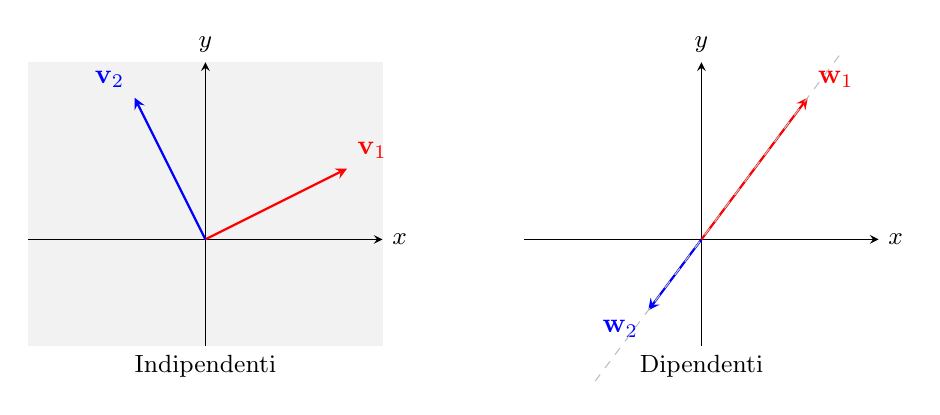
\begin{tikzpicture}[>=stealth, scale=0.9]
    % Left: Independent
    \begin{scope}
        \fill[gray!10] (-2.5,-1.5) rectangle (2.5,2.5);
        \draw[->] (-2.5,0) -- (2.5,0) node[right]{\small $x$};
        \draw[->] (0,-1.5) -- (0,2.5) node[above]{\small $y$};
        \draw[->, thick, red] (0,0) -- (2,1) node[above right]{$\mathbf{v}_1$};
        \draw[->, thick, blue] (0,0) -- (-1,2) node[above left]{$\mathbf{v}_2$};
        \node[below] at (0,-1.5) {\small Indipendenti};
    \end{scope}
    % Right: Dependent
    \begin{scope}[xshift=7cm]
        \draw[->] (-2.5,0) -- (2.5,0) node[right]{\small $x$};
        \draw[->] (0,-1.5) -- (0,2.5) node[above]{\small $y$};
        \draw[->, thick, red] (0,0) -- (1.5,2) node[above right]{$\mathbf{w}_1$};
        \draw[->, thick, blue] (0,0) -- (-0.75,-1) node[below left]{$\mathbf{w}_2$};
        \draw[dashed, gray!50] (-1.5,-2) -- (2,2.67);
        \node[below] at (0,-1.5) {\small Dipendenti};
    \end{scope}
\end{tikzpicture}
\caption{Vettori linearmente indipendenti (a sinistra) e dipendenti (a destra) in $\mathbb{R}^2$.}
\label{fig:indipendenza}
\end{figure}

\section{Basi e dimensione}
\label{sec:basi-dimensione}

\begin{definitionbox}[Base]
Un insieme di vettori $\mathcal{B} = \{\mathbf{v}_1, \ldots, \mathbf{v}_n\}$ è una \textbf{base} di $V$ se:
\begin{enumerate}
    \item $\mathcal{B}$ è un sistema di generatori di $V$;
    \item $\mathcal{B}$ è linearmente indipendente.
\end{enumerate}
Equivalentemente, $\mathcal{B}$ è una base se ogni $\mathbf{v} \in V$ si scrive in modo \emph{unico} come combinazione lineare degli elementi di $\mathcal{B}$.
\end{definitionbox}

\begin{examplebox}[Base canonica di $\mathbb{R}^n$]
La \textbf{base canonica} di $\mathbb{R}^n$ è $\{\mathbf{e}_1, \mathbf{e}_2, \ldots, \mathbf{e}_n\}$ dove:
\[ \mathbf{e}_1 = (1,0,\ldots,0), \;\; \mathbf{e}_2 = (0,1,\ldots,0), \;\; \ldots, \;\; \mathbf{e}_n = (0,0,\ldots,1). \]
Ogni $\mathbf{v} = (v_1, \ldots, v_n) \in \mathbb{R}^n$ si scrive come $\mathbf{v} = v_1\mathbf{e}_1 + \cdots + v_n\mathbf{e}_n$.
\end{examplebox}

\begin{theorembox}[Teorema della base (Steinitz)]
\label{thm:steinitz}
Sia $V$ uno spazio vettoriale finitamente generato. Allora:
\begin{enumerate}
    \item $V$ ammette almeno una base.
    \item Tutte le basi di $V$ hanno lo stesso numero di elementi.
    \item Ogni insieme linearmente indipendente può essere esteso a una base.
    \item Da ogni sistema di generatori si può estrarre una base.
\end{enumerate}
\end{theorembox}

\begin{definitionbox}[Dimensione]
La \textbf{dimensione} di uno spazio vettoriale $V$, indicata con $\dim V$, è il numero di elementi di una qualsiasi base di $V$. Per convenzione, $\dim\{\mathbf{0}\} = 0$.
\end{definitionbox}

\begin{examplebox}[Dimensioni notevoli]
\begin{itemize}
    \item $\dim \mathbb{R}^n = n$
    \item $\dim \mathcal{M}_{m \times n}(\mathbb{R}) = mn$
    \item $\dim \mathbb{R}[x]_{\leq n} = n + 1$
\end{itemize}
\end{examplebox}

\begin{figure}[htbp]
  \centering
  
\includegraphics[width=0.75\textwidth]{ch01-canonical-basis}
  \caption{La base canonica $\{\mathbf{e}_1, \mathbf{e}_2, \mathbf{e}_3\}$ di $\mathbb{R}^3$ e la decomposizione di un vettore $\mathbf{v}$ come combinazione lineare dei vettori di base.}
  \label{fig:ch01-canonical-basis}
\end{figure}

\begin{theorembox}[Criterio di base per dimensione]
\label{thm:criterio-base}
Sia $\dim V = n$. Allora:
\begin{enumerate}
    \item $n$ vettori linearmente indipendenti formano una base.
    \item $n$ vettori che generano $V$ formano una base.
    \item Più di $n$ vettori sono sempre linearmente dipendenti.
    \item Meno di $n$ vettori non possono generare $V$.
\end{enumerate}
\end{theorembox}

\begin{definitionbox}[Coordinate rispetto a una base]
Sia $\mathcal{B} = \{\mathbf{v}_1, \ldots, \mathbf{v}_n\}$ una base di $V$. Se $\mathbf{v} = \lambda_1\mathbf{v}_1 + \cdots + \lambda_n\mathbf{v}_n$, il vettore colonna
\[ [\mathbf{v}]_{\mathcal{B}} = \begin{pmatrix} \lambda_1 \\ \vdots \\ \lambda_n \end{pmatrix} \in \mathbb{R}^n \]
è il \textbf{vettore delle coordinate} di $\mathbf{v}$ rispetto alla base $\mathcal{B}$.
\end{definitionbox}

\begin{examplebox}[Coordinate in una base non canonica]
In $\mathbb{R}^2$, consideriamo la base $\mathcal{B} = \{(1,1), (1,-1)\}$. Troviamo le coordinate di $\mathbf{v} = (3, 1)$ rispetto a $\mathcal{B}$. Dobbiamo risolvere:
\[ \lambda_1(1,1) + \lambda_2(1,-1) = (3,1) \quad \Longrightarrow \quad \begin{cases} \lambda_1 + \lambda_2 = 3 \\ \lambda_1 - \lambda_2 = 1 \end{cases} \]
Da cui $\lambda_1 = 2$, $\lambda_2 = 1$. Quindi $[\mathbf{v}]_{\mathcal{B}} = \begin{pmatrix} 2 \\ 1 \end{pmatrix}$.
\end{examplebox}

\begin{notebox}[Riepilogo del capitolo]
In questo capitolo abbiamo introdotto le strutture fondamentali dell'algebra lineare:
\begin{itemize}
    \item Lo \textbf{spazio vettoriale} come struttura algebrica con somma e prodotto per scalare.
    \item I \textbf{sottospazi} come ``sotto-ambienti'' chiusi per combinazioni lineari.
    \item L'\textbf{indipendenza lineare} come criterio di non-ridondanza.
    \item Le \textbf{basi} e la \textbf{dimensione} come misura della ``grandezza'' di uno spazio.
\end{itemize}
Questi concetti saranno utilizzati in modo sistematico nei capitoli successivi.
\end{notebox}
